\section{Resultados}

\subsection{Segunda Consigna: Gráficos y Análisis}

\subsubsection{Red Doméstica}

Para la primera captura, se eligió una red domestica de uno de los integrantes del grupo.
La captura duro 30 minutos aproximados.
Al ser una red pequeña podemos distinguir fácilmente los nodos destacados.
La Figura~\ref{fig:red_domestica_network}. muestra 2 nodos destacados 192.168.0.1 que correspondes al router  y el nodo 192.168.0.27 correspondiente al PC desde donde se tomaron las capturas.

\begin{figure}[h!]
  \centering
   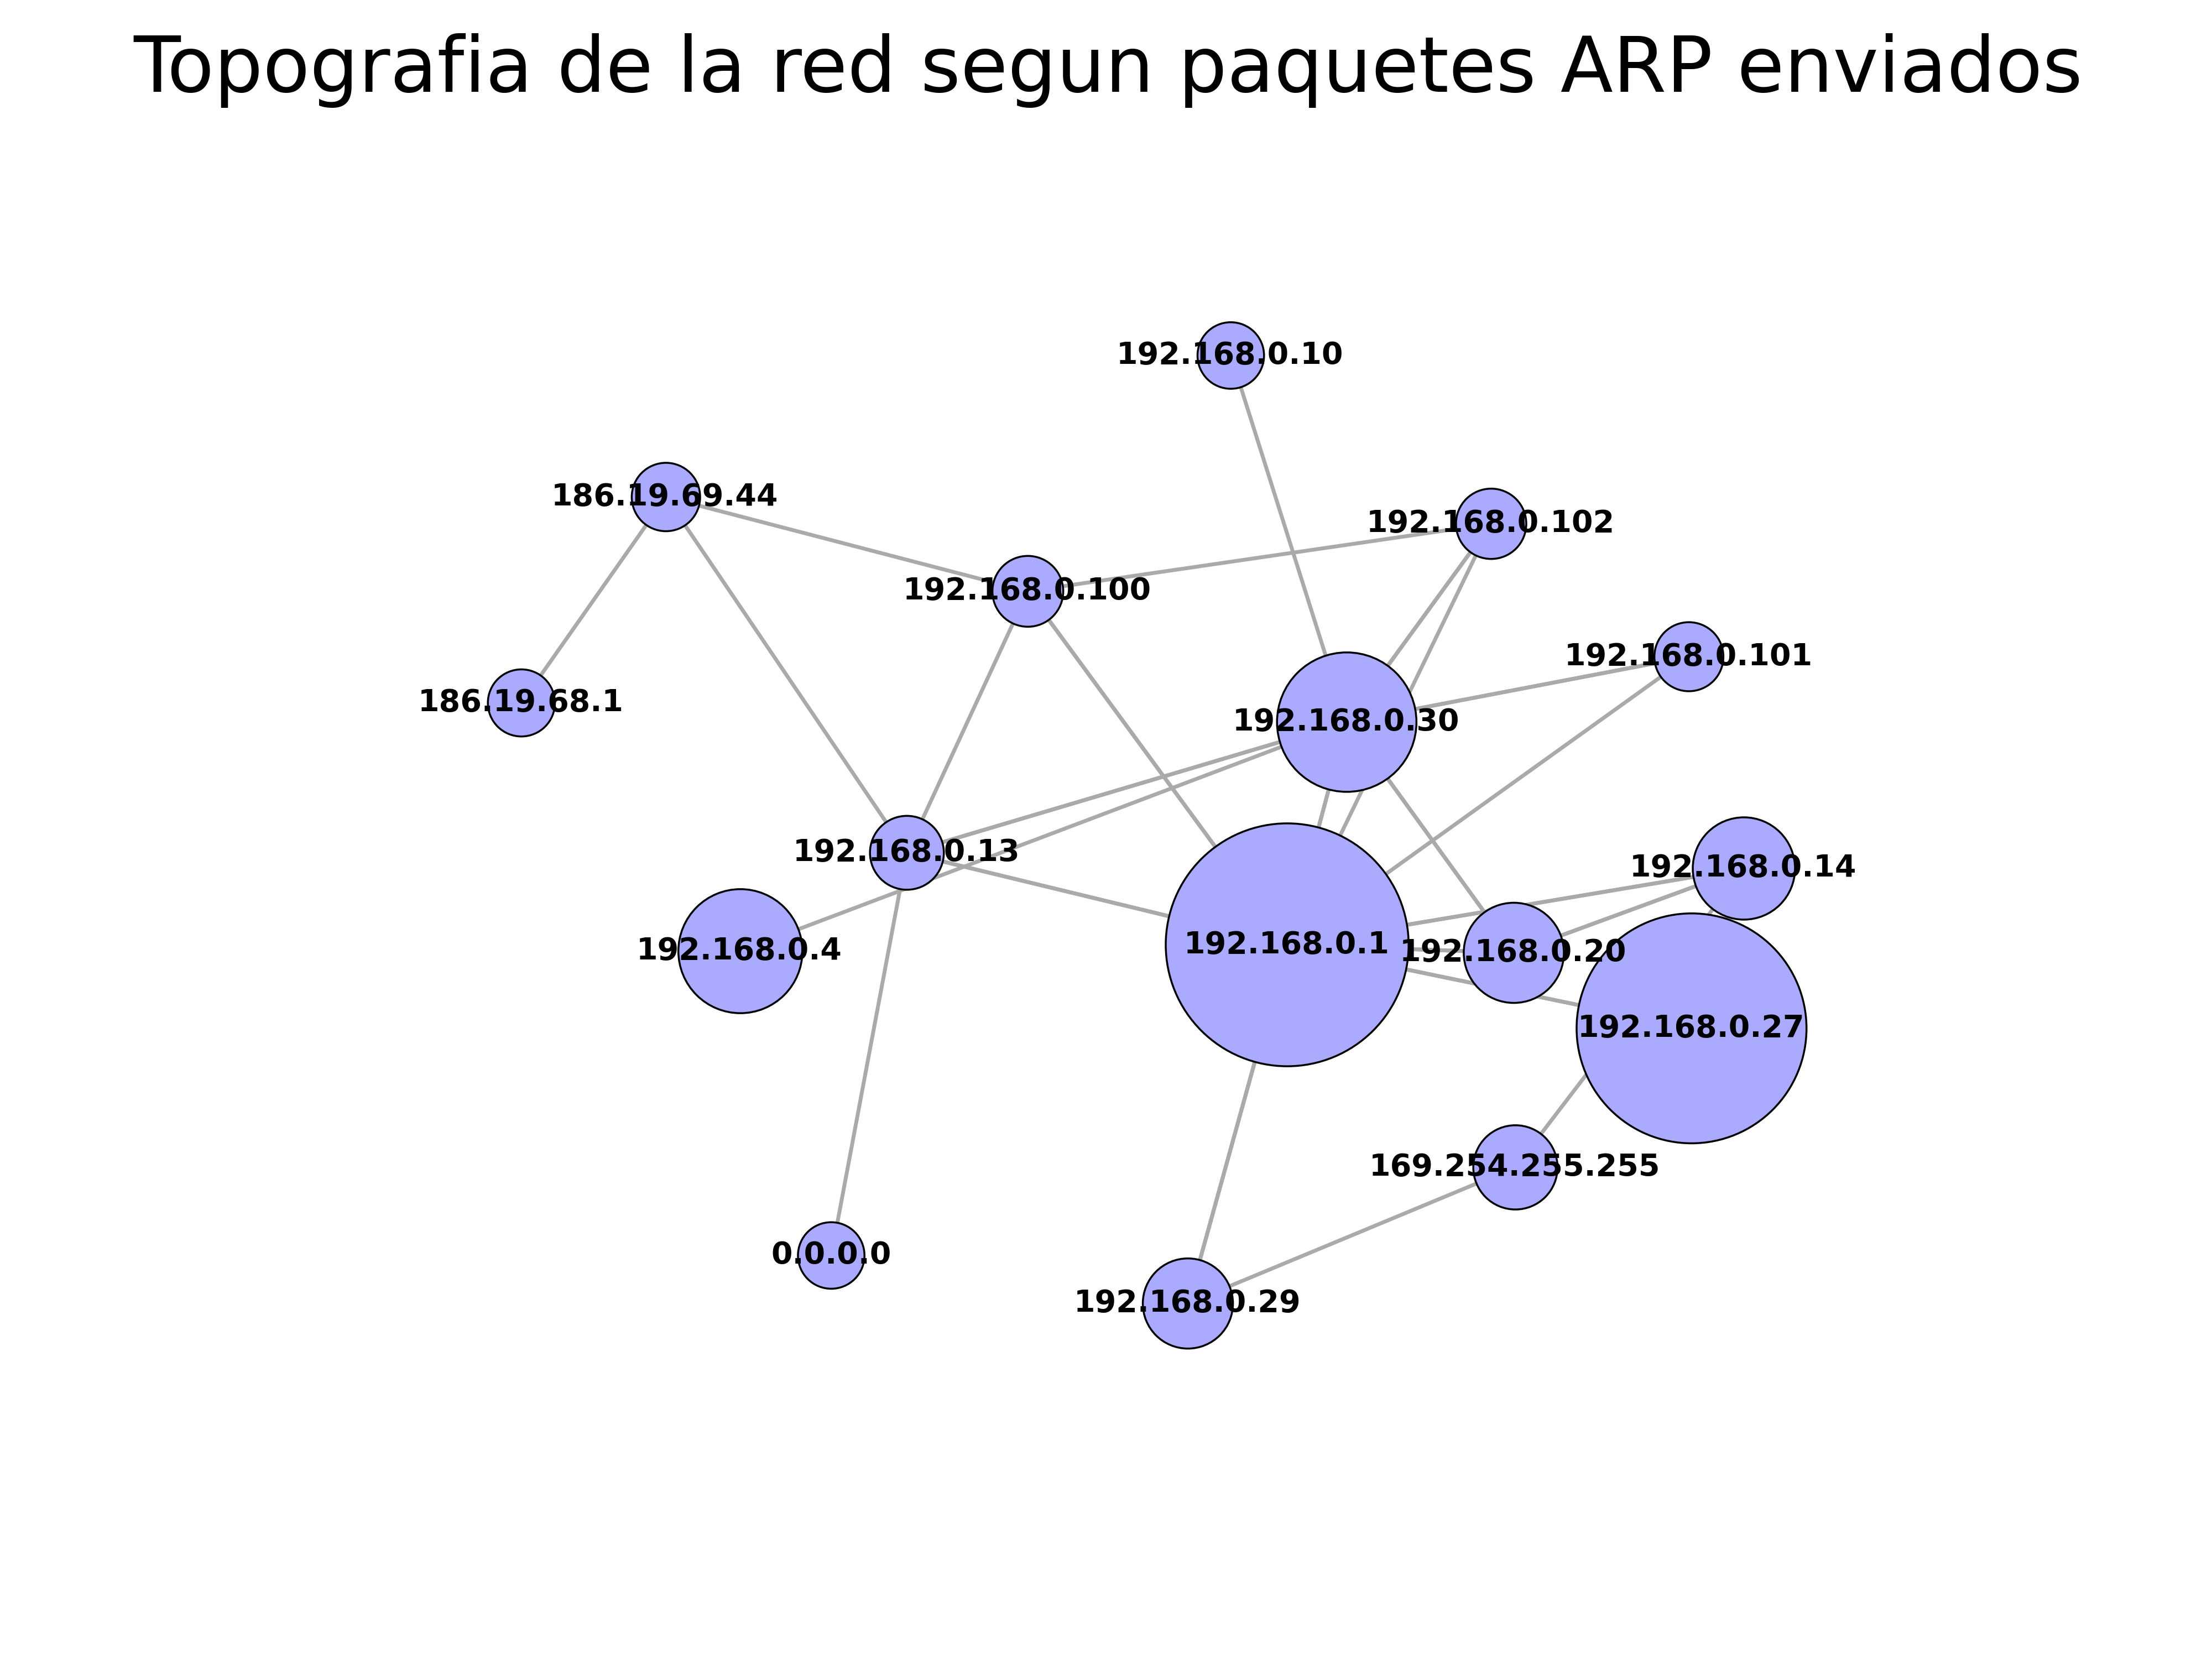
\includegraphics[width=0.7\textwidth]{graficos/red_domestica_network.png}}
  \caption{Mi Figura}
  \label{fig:red_domestica_network}
\end{figure}

\FloatBarrier

\subsubsection{Histogramas (de IPs y protocolos)}

\begin{figure}
  \centering
   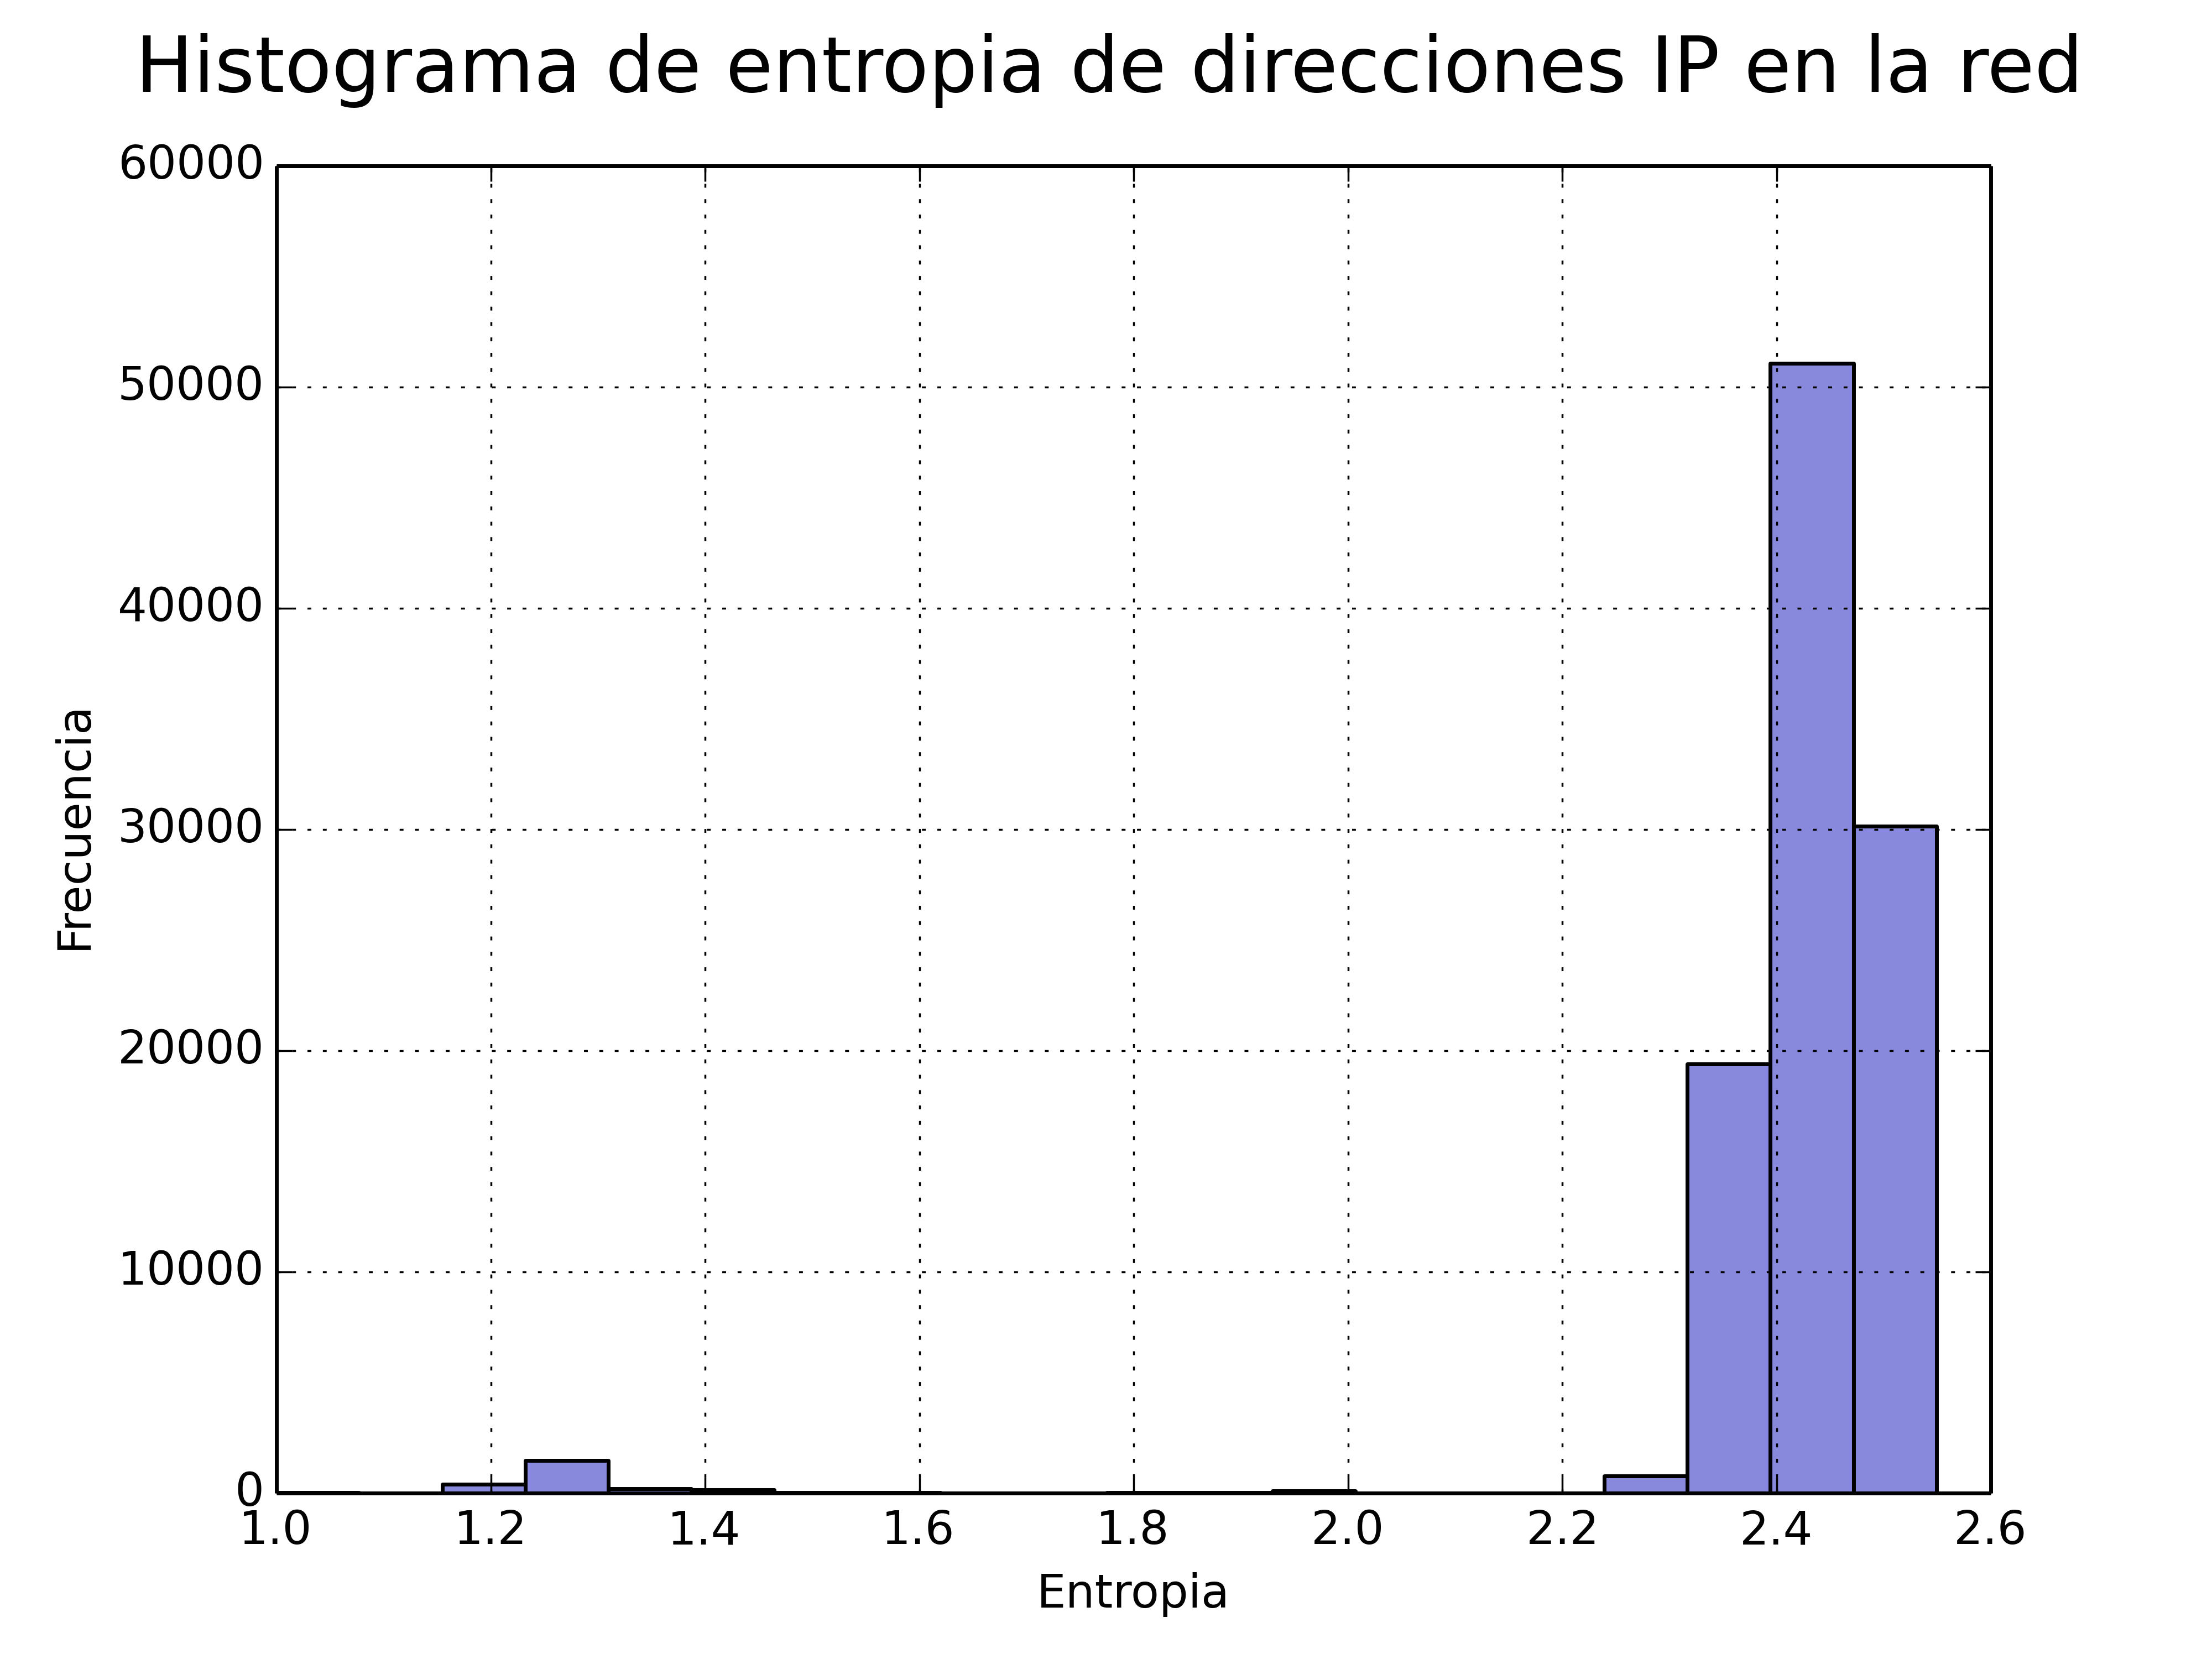
\includegraphics[width=0.7\textwidth]{graficos/red_domestica_hist_arp.png}}
  \caption{Mi Figura}
  \label{fig:ejemplo}
\end{figure}

\begin{figure}
  \centering
   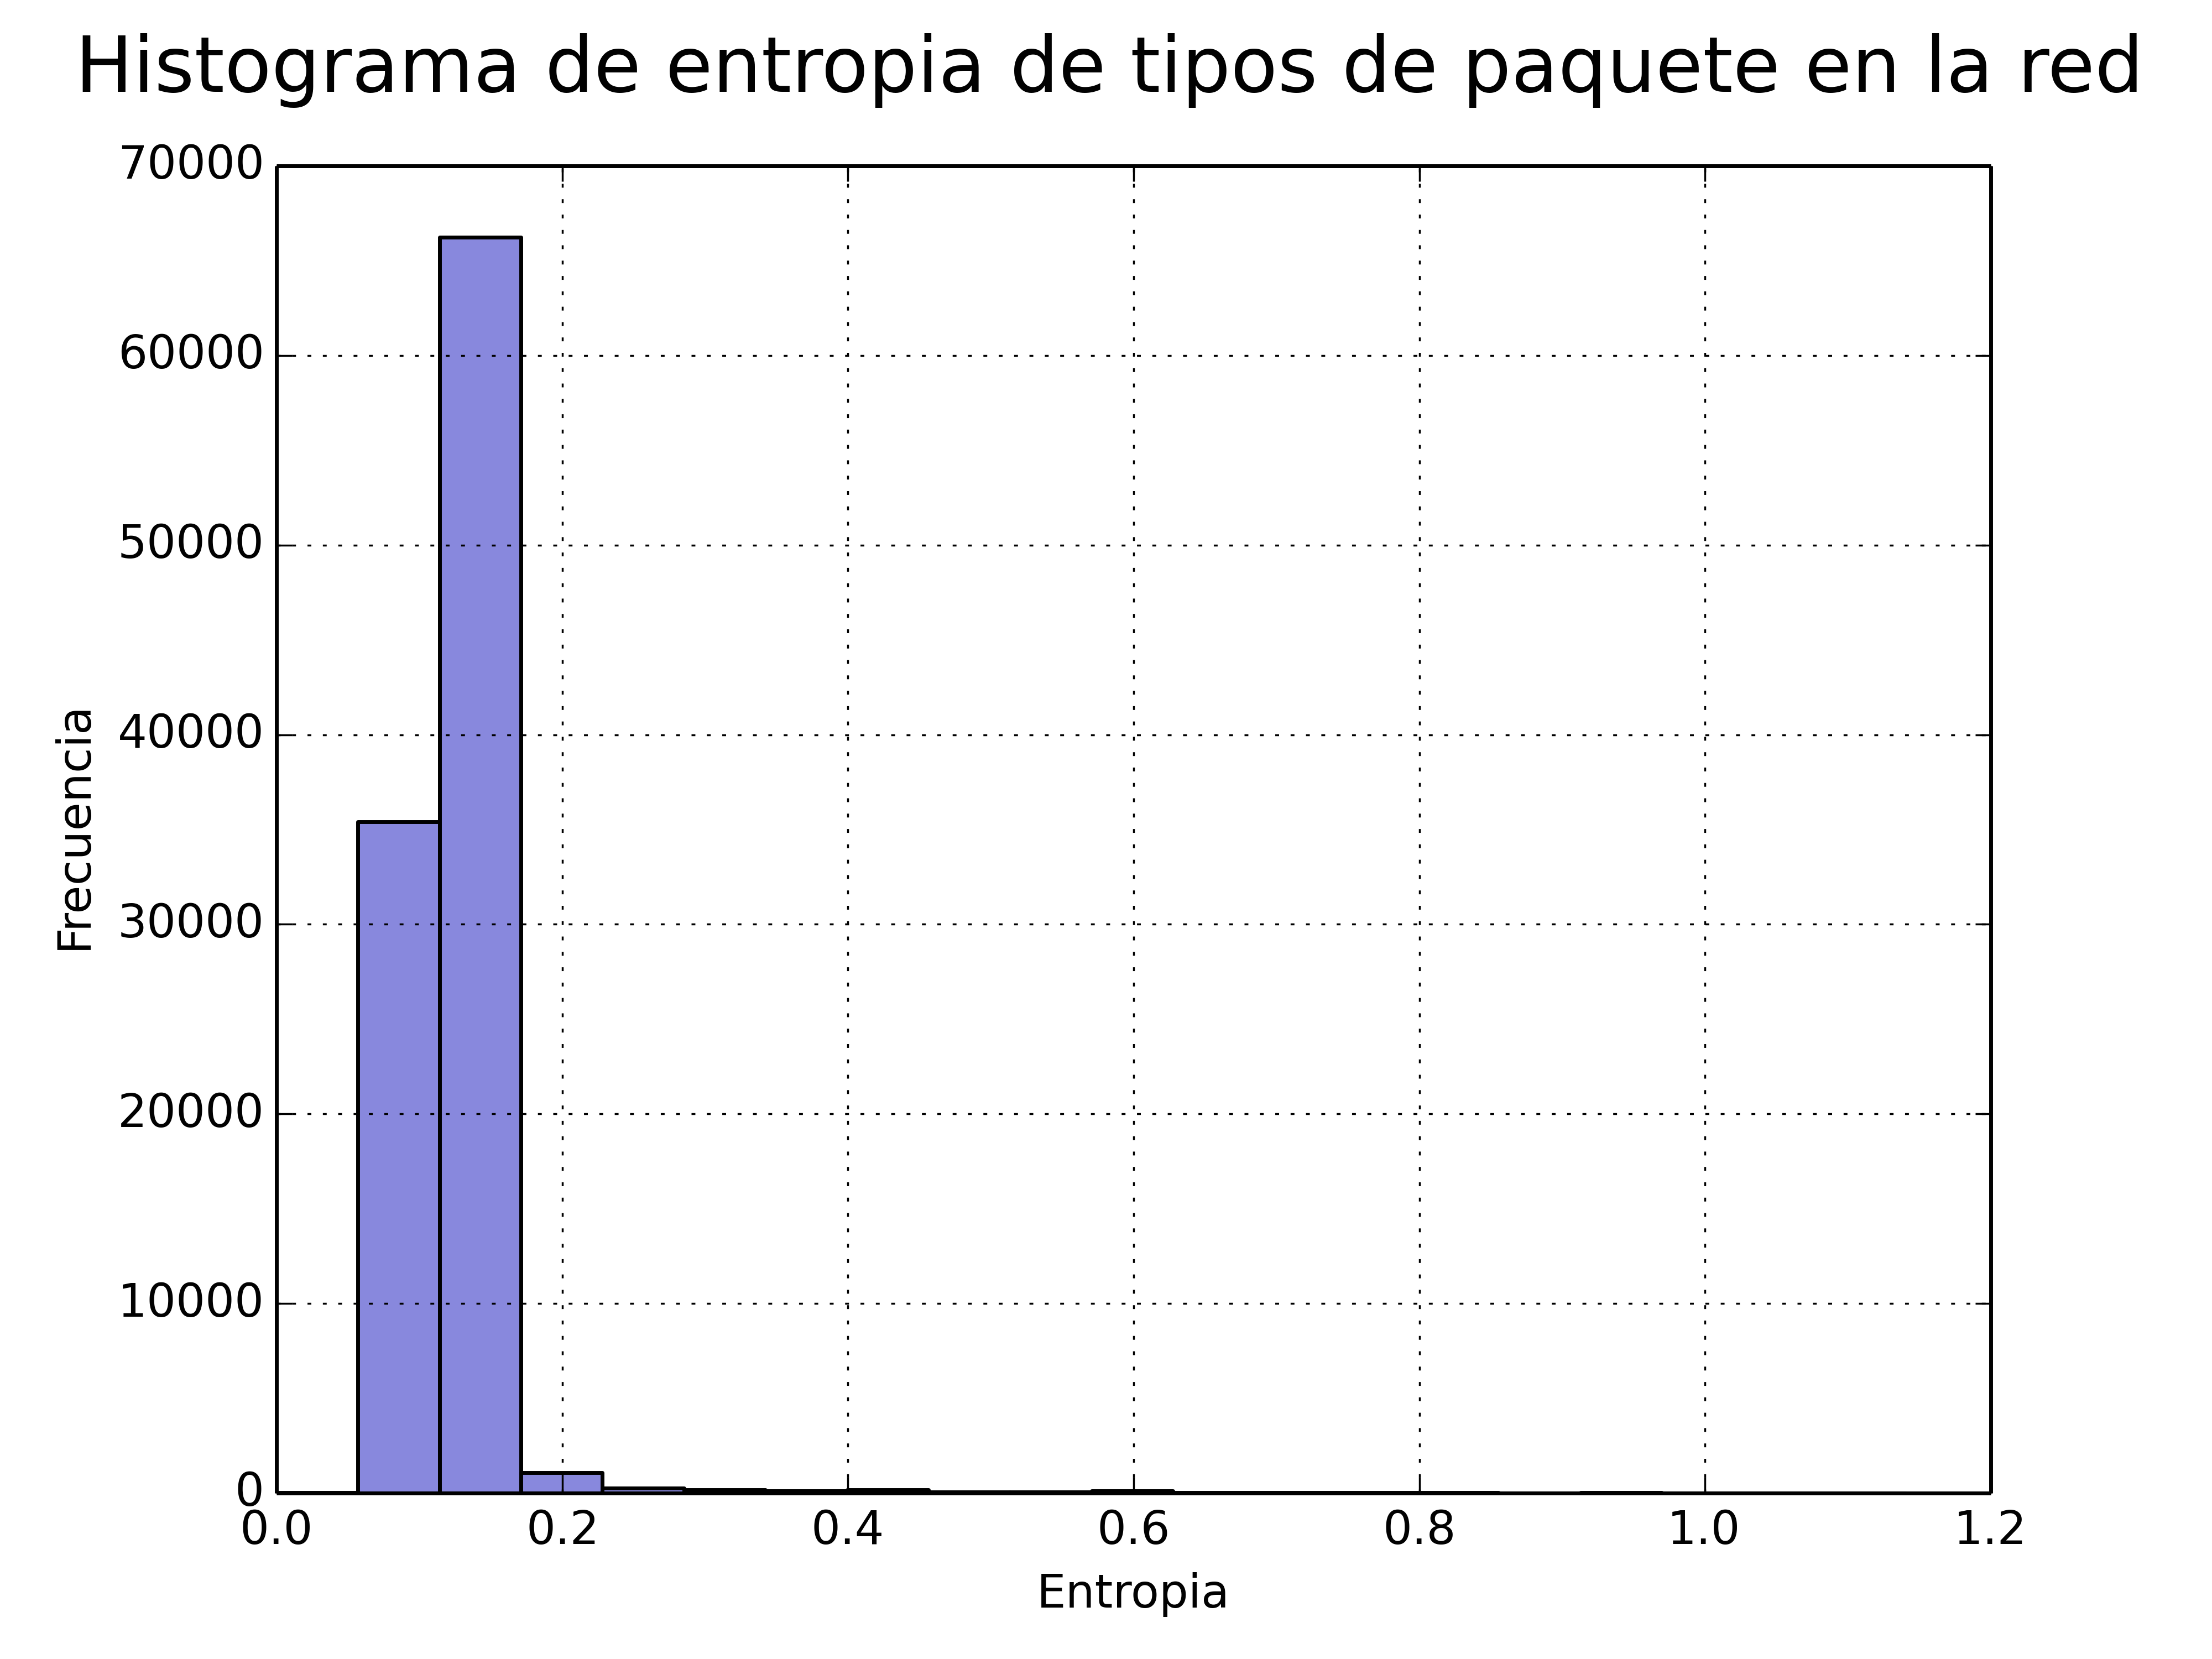
\includegraphics[width=0.7\textwidth]{graficos/red_domestica_hist_type.png}}
  \caption{Mi Figura}
  \label{fig:ejemplo}
\end{figure}

\FloatBarrier

\subsubsection{Paquetes capturados e información}

\begin{figure}
  \centering
   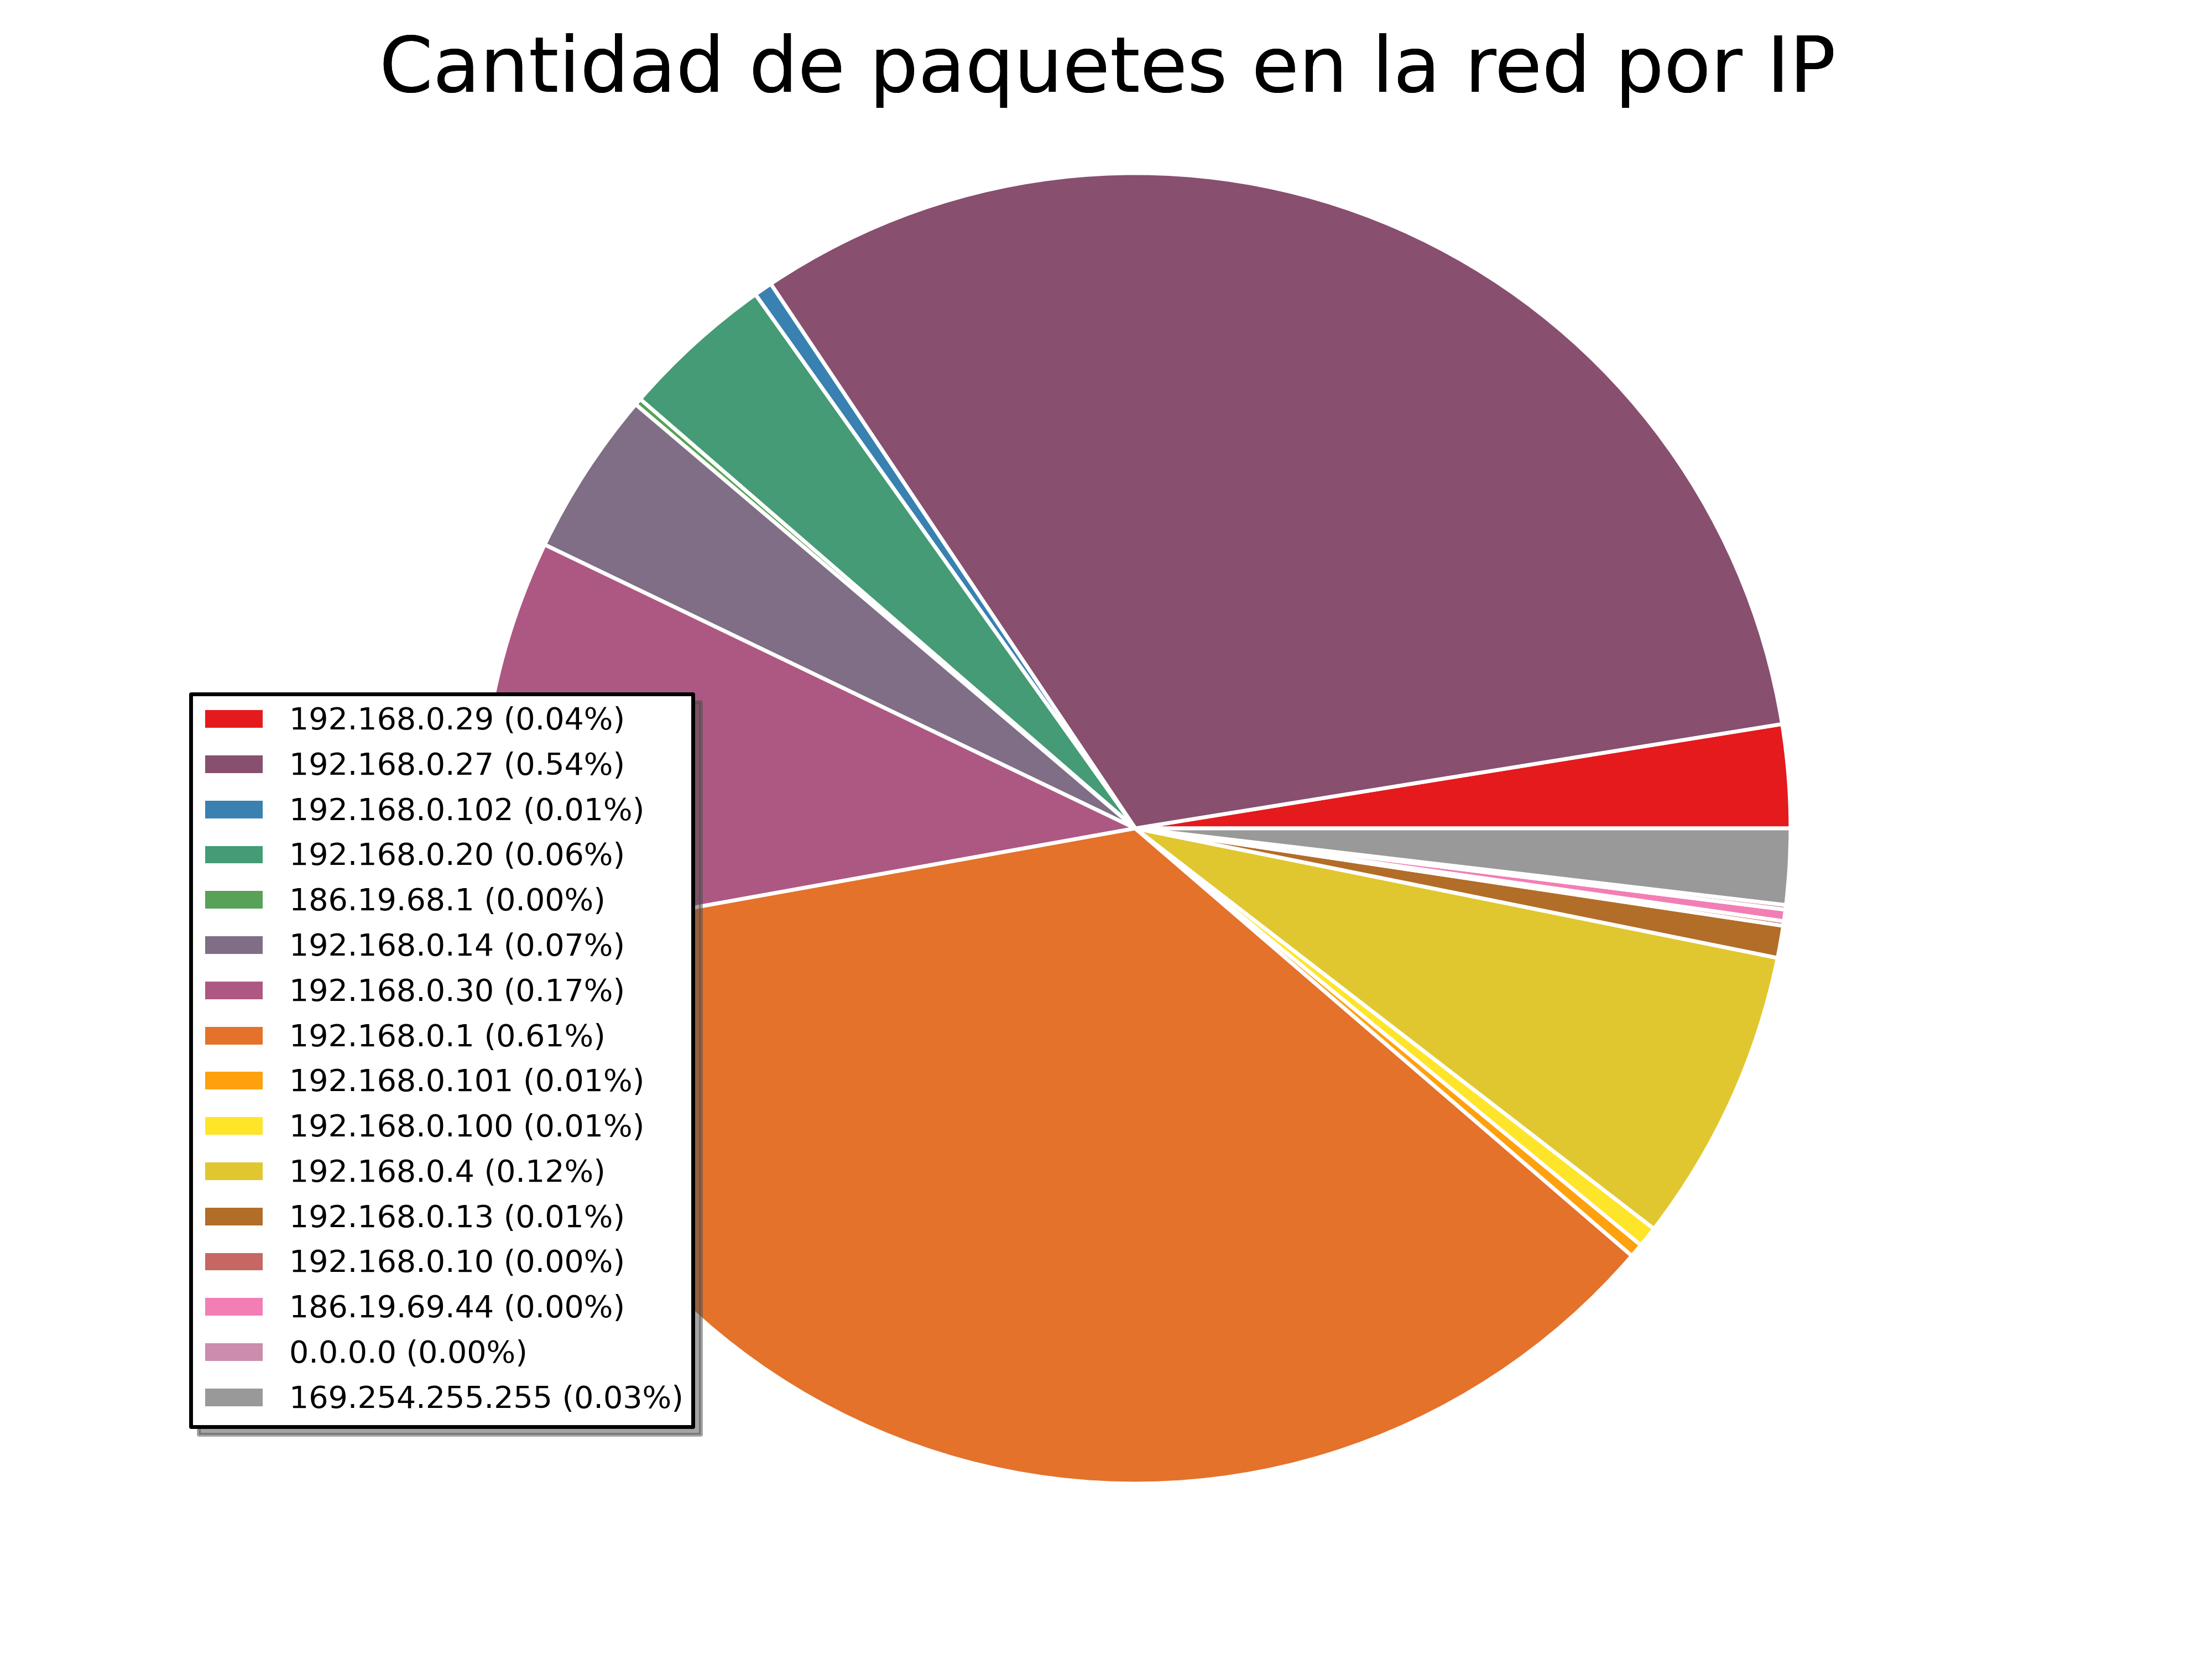
\includegraphics[width=0.7\textwidth]{graficos/red_domestica_pie_arp.png}}
  \caption{Mi Figura}
  \label{fig:ejemplo}
\end{figure}

\begin{figure}
  \centering
   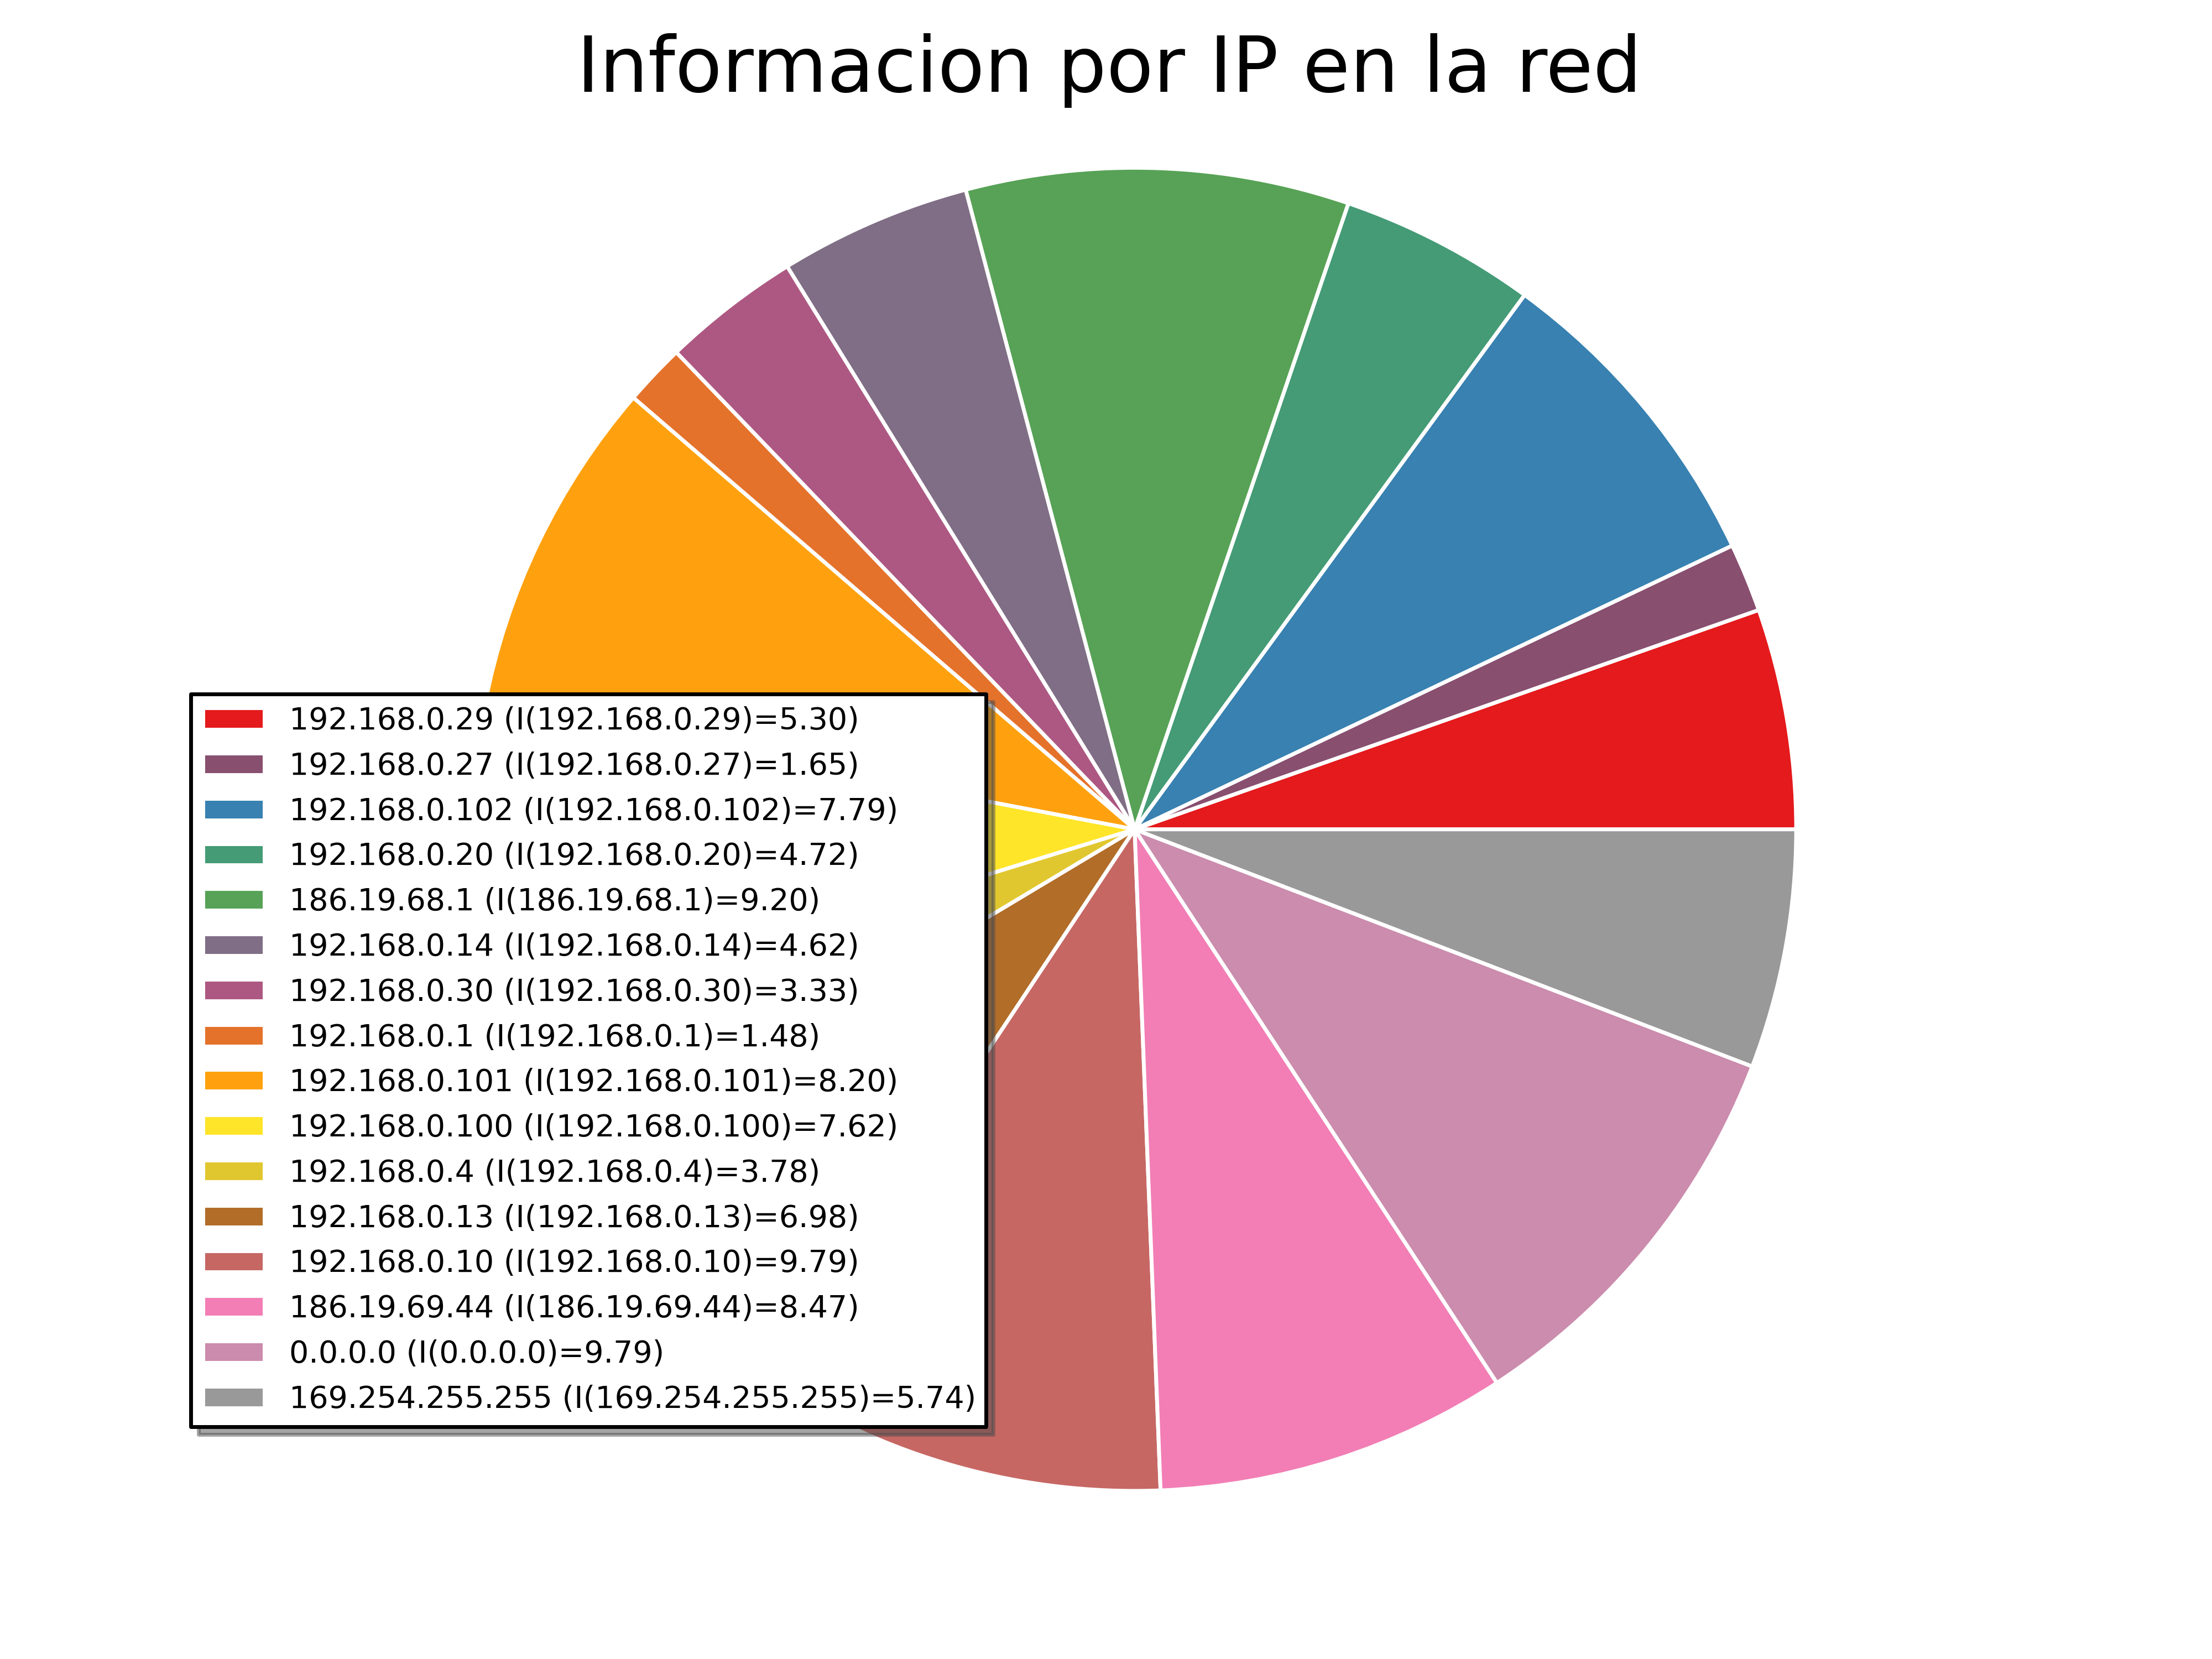
\includegraphics[width=0.7\textwidth]{graficos/red_domestica_pie_arp_information.png}}
  \caption{Mi Figura}
  \label{fig:ejemplo}
\end{figure}

\begin{figure}
  \centering
   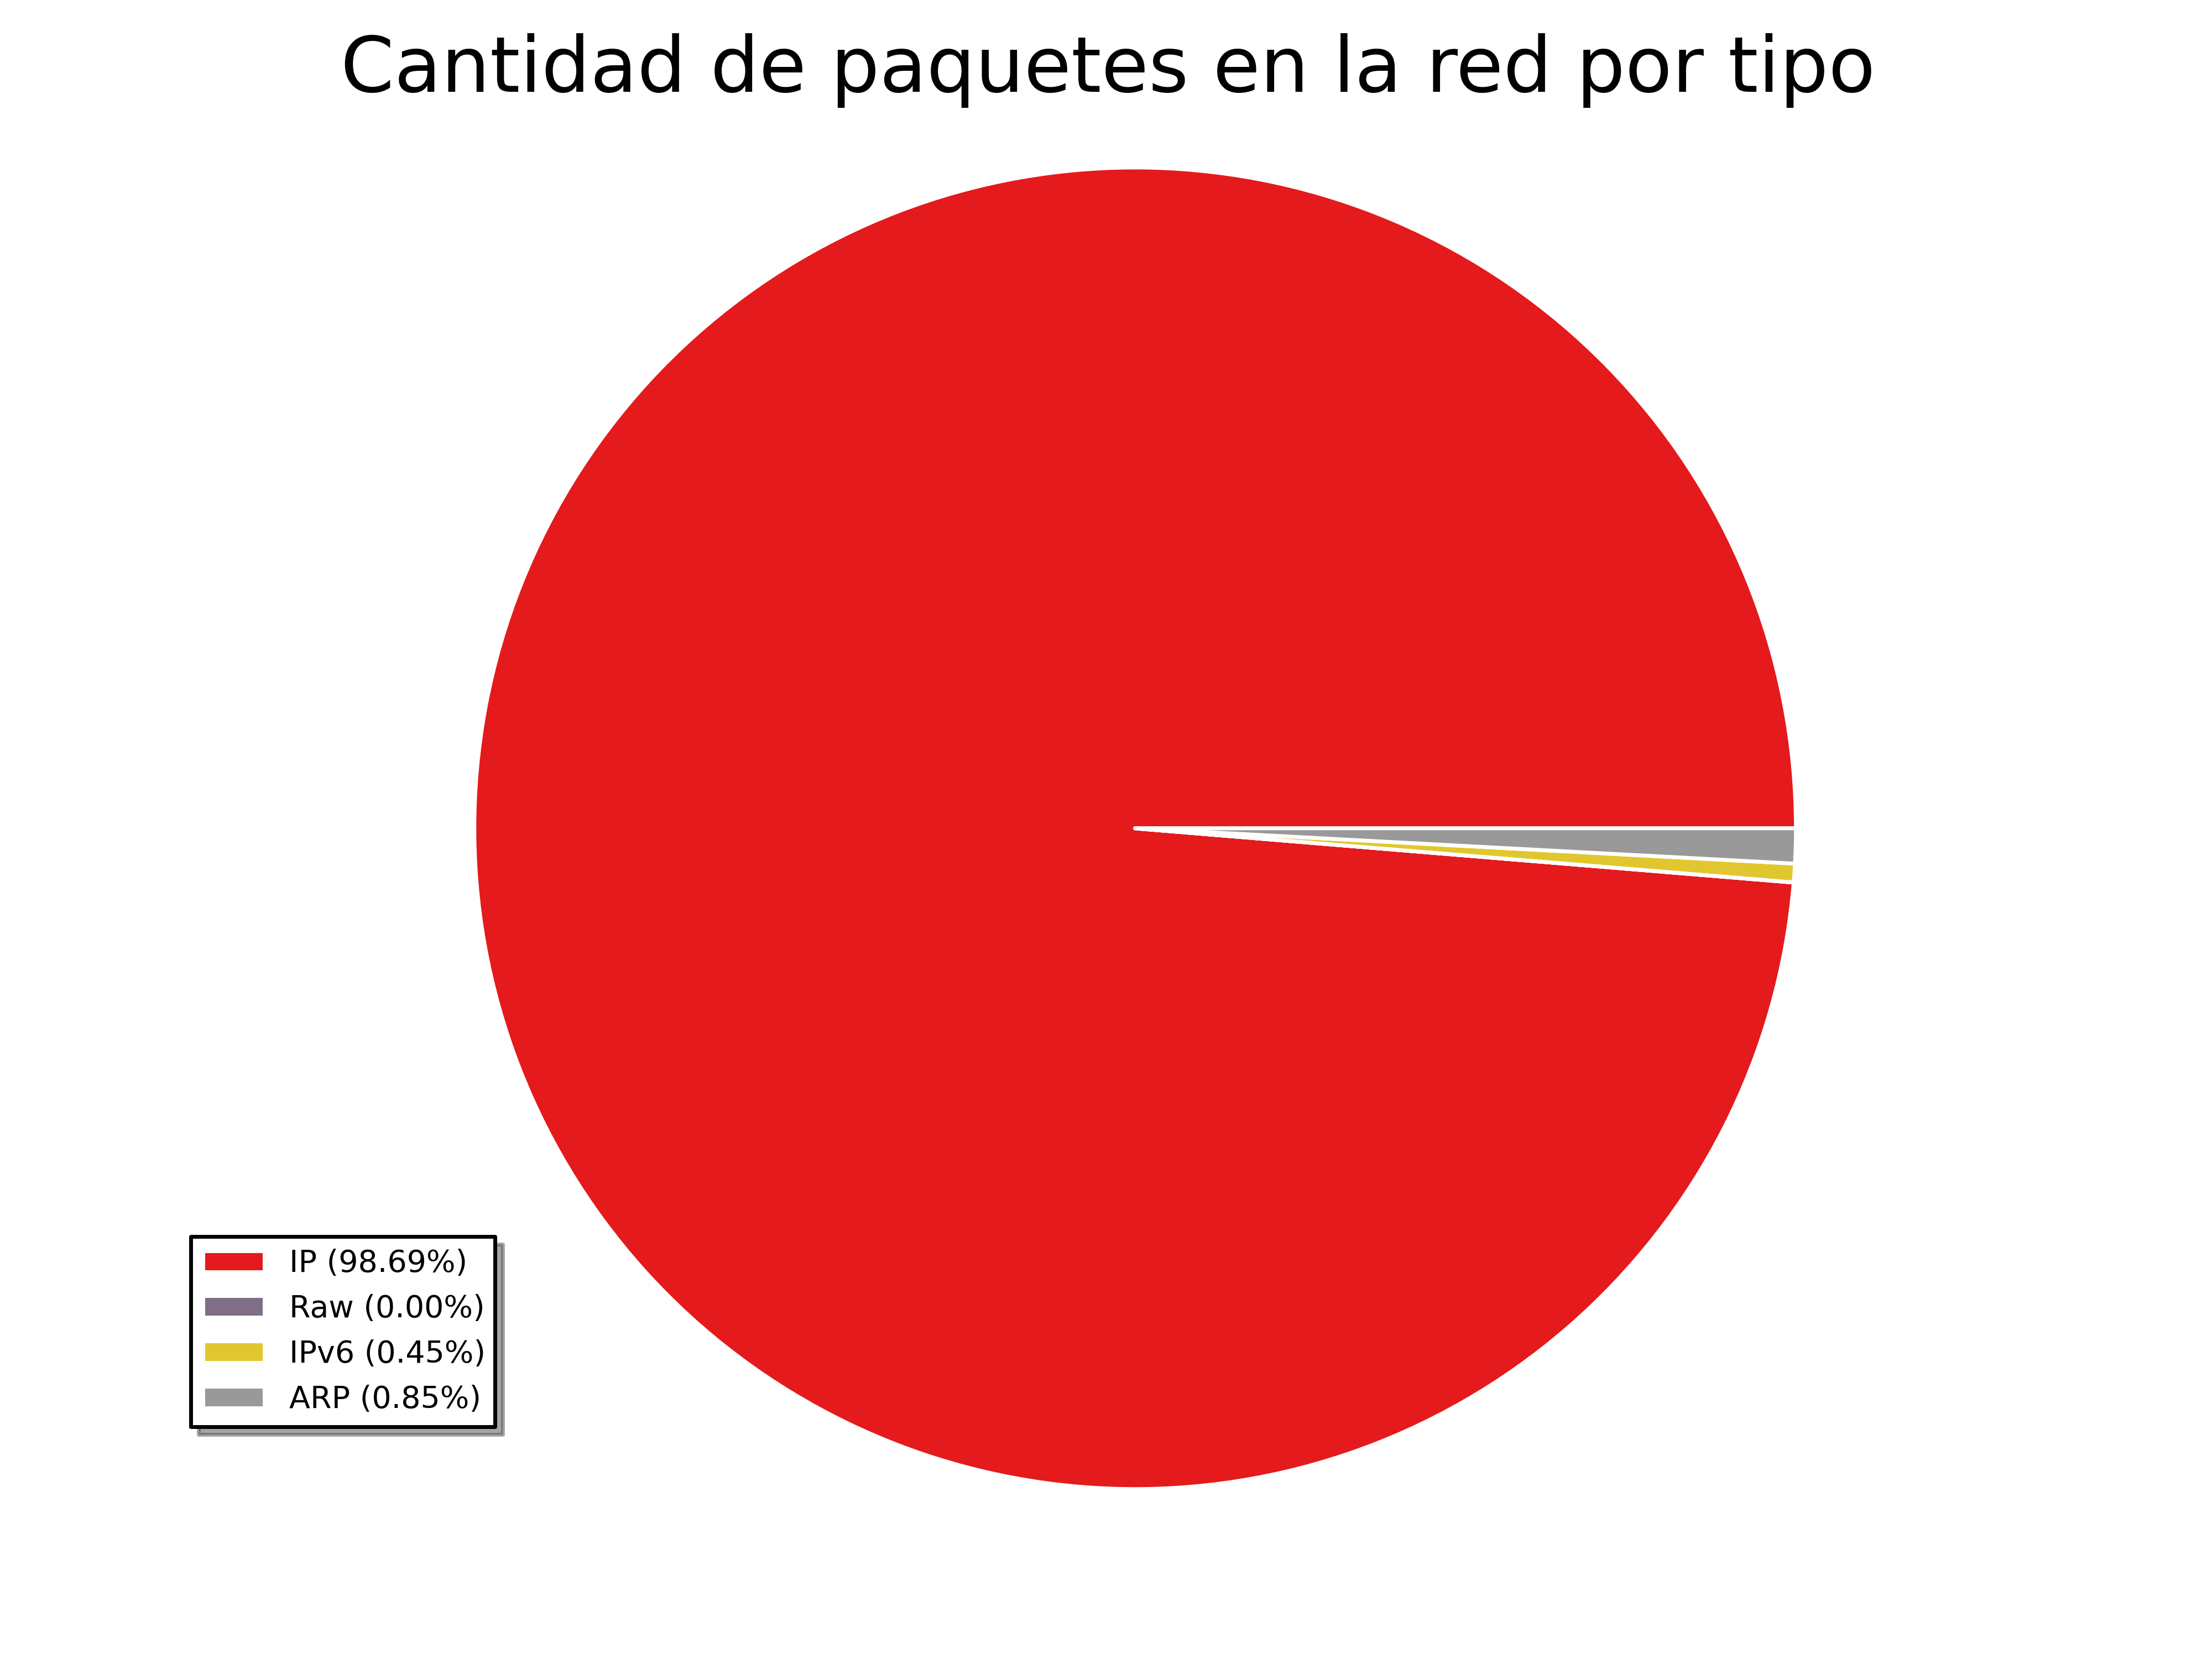
\includegraphics[width=0.7\textwidth]{graficos/red_domestica_pie_type.png}}
  \caption{Mi Figura}
  \label{fig:ejemplo}
\end{figure}

\begin{figure}
  \centering
   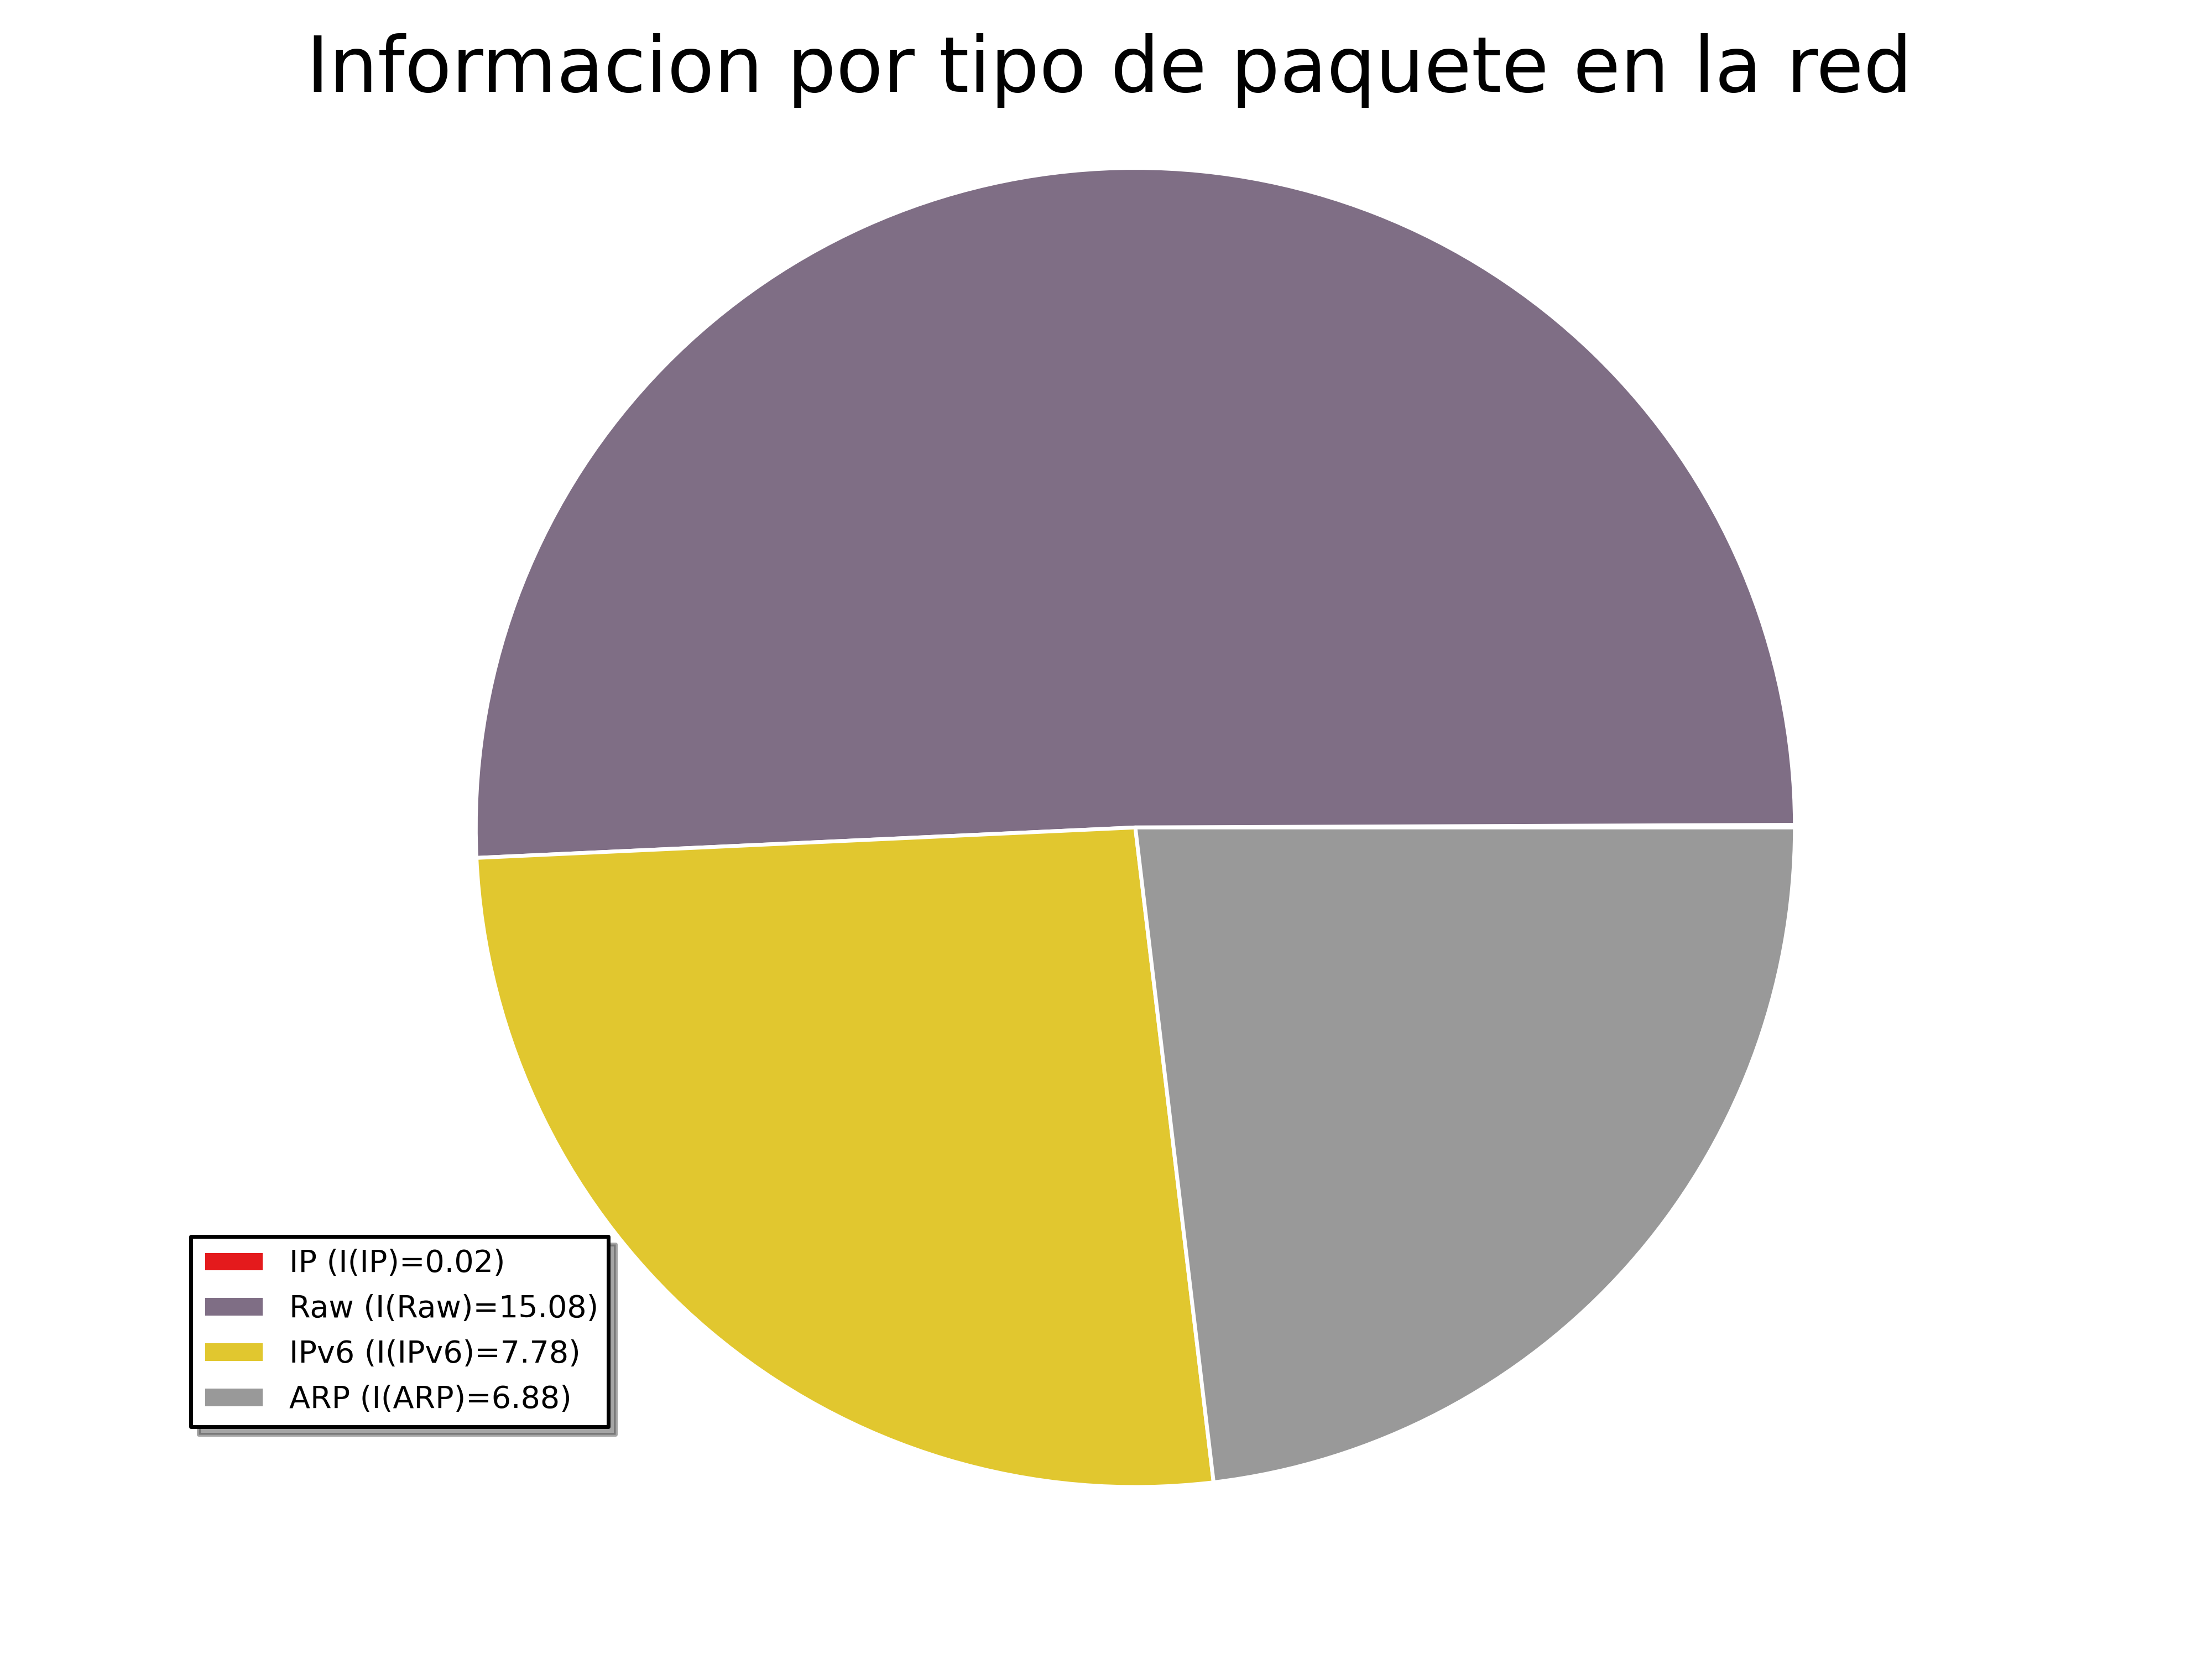
\includegraphics[width=0.7\textwidth]{graficos/red_domestica_pie_type_information.png}}
  \caption{Mi Figura}
  \label{fig:ejemplo}
\end{figure}